\documentclass[margin=3cm,mikulas,portrait,final]{myposter}
%\documentclass[a4shrink,portrait,final]{baposter}
% Usa a4shrink for an a4 sized paper.

\tracingstats=2

\usepackage{times}
\usepackage{calc}
\usepackage[intlimits]{amsmath}
\usepackage{amssymb}
\usepackage{relsize}
\usepackage{multirow}
\usepackage{bm}

\usepackage[czech]{babel}
\usepackage[utf8]{inputenc}

\usepackage{graphicx}
\usepackage{multicol}
%\usepackage{wasysym}


\usepackage{nicefrac}
\usetikzlibrary{positioning,calc,arrows,snakes,backgrounds,patterns,shapes,fit,shadows,plotmarks}

\usepackage{pgfbaselayers}
\pgfdeclarelayer{background}
\pgfdeclarelayer{midground}
\pgfdeclarelayer{foreground}
\pgfsetlayers{background,midground,main,foreground}

\usepackage{helvet}
%\usepackage{bookman}
\usepackage{palatino}

\selectcolormodel{cmyk}

\graphicspath{{obr/}}

%%%%%%%%%%%%%%%%%%%%%%%%%%%%%%%%%%%%%%%%%%%%%%%%%%%%%%%%%%%%%%%%%%%%%%%%%%%%%%%%
%%%% Some math symbols used in the text
%%%%%%%%%%%%%%%%%%%%%%%%%%%%%%%%%%%%%%%%%%%%%%%%%%%%%%%%%%%%%%%%%%%%%%%%%%%%%%%%
% Format 
\newcommand{\Matrix}[1]{\begin{bmatrix} #1 \end{bmatrix}}
\newcommand{\Vector}[1]{\Matrix{#1}}
\newcommand*{\SET}[1]{\ensuremath{\mathcal{#1}}}
\newcommand*{\MAT}[1]{\ensuremath{\mathbf{#1}}}
\newcommand*{\VEC}[1]{\ensuremath{\bm{#1}}}
\newcommand*{\CONST}[1]{\ensuremath{\mathit{#1}}}
\newcommand*{\norm}[1]{\mathopen\Vert #1 \mathclose\Vert}
\newcommand*{\abs}[1]{\mathopen| #1 \mathclose|}
\newcommand*{\absLR}[1]{\left| #1 \right|}

\def\norm#1{\mathopen\| #1 \mathclose\|}
\newcommand{\normLR}[1]{\left\| #1 \right\|}

\newcommand{\restrict}[2]{\left.#1\right\vert_{#2}}
\renewcommand{\it}[1]{^{(#1)}}
\newcommand{\nod}{^{\mathrm{nod}}}
\newcommand{\iterace}{i}
\newcommand{\LP}{L\!\mid\!P}
\renewcommand{\DH}{D\!\mid\!H}
\newcommand{\captionfont}{\footnotesize}
\newcommand{\keff}{k_{\mathrm{eff}}}
\newcommand{\suma}{\sum_{\makebox[0pt]{${\scriptscriptstyle{g'\neq g}}$}}}
\newcommand{\bj}{\mathbf{j}}
\newcommand{\phinod}{\varphi(x)}
\newcommand{\dphidx}[1][]{\frac{d^{#1}\phinod}{dx^{#1}}}


%%%%%%%%%%%%%%%%%%%%%%%%%%%%%%%%%%%%%%%%%%%%%%%%%%%%%%%%%%%%%%%%%%%%%%%%%%%%%%%%
% Multicol Settings
%%%%%%%%%%%%%%%%%%%%%%%%%%%%%%%%%%%%%%%%%%%%%%%%%%%%%%%%%%%%%%%%%%%%%%%%%%%%%%%%
\setlength{\columnsep}{0.7em}
\setlength{\columnseprule}{0mm}


%%%%%%%%%%%%%%%%%%%%%%%%%%%%%%%%%%%%%%%%%%%%%%%%%%%%%%%%%%%%%%%%%%%%%%%%%%%%%%%%
% Save space in lists. Use this after the opening of the list
%%%%%%%%%%%%%%%%%%%%%%%%%%%%%%%%%%%%%%%%%%%%%%%%%%%%%%%%%%%%%%%%%%%%%%%%%%%%%%%%
\newcommand{\compresslist}{%
\setlength{\itemsep}{1pt}%
\setlength{\parskip}{0pt}%
\setlength{\parsep}{0pt}%
}


%%%%%%%%%%%%%%%%%%%%%%%%%%%%%%%%%%%%%%%%%%%%%%%%%%%%%%%%%%%%%%%%%%%%%%%%%%%%%%
%%% Begin of Document
%%%%%%%%%%%%%%%%%%%%%%%%%%%%%%%%%%%%%%%%%%%%%%%%%%%%%%%%%%%%%%%%%%%%%%%%%%%%%%

\begin{document}
\pagestyle{empty}
%%%%%%%%%%%%%%%%%%%%%%%%%%%%%%%%%%%%%%%%%%%%%%%%%%%%%%%%%%%%%%%%%%%%%%%%%%%%%%
%%% Here starts the poster
%%%---------------------------------------------------------------------------
%%% Format it to your taste with the options
%%%%%%%%%%%%%%%%%%%%%%%%%%%%%%%%%%%%%%%%%%%%%%%%%%%%%%%%%%%%%%%%%%%%%%%%%%%%%%
% Define some colors
\definecolor{silver}{cmyk}{0,0,0,0.3}
\definecolor{yellow}{cmyk}{0,0,0.9,0.0}
\definecolor{reddishyellow}{cmyk}{0,0.22,1.0,0.0}
\definecolor{black}{cmyk}{0,0,0.0,1.0}
\definecolor{darkYellow}{cmyk}{0,0,1.0,0.5}
\definecolor{darkSilver}{cmyk}{0,0,0,0.1}

\definecolor{lightyellow}{cmyk}{0,0,0.3,0.0}
\definecolor{lighteryellow}{cmyk}{0,0,0.1,0.0}
\definecolor{lightestyellow}{cmyk}{0,0,0.05,0.0}


%%
\typeout{Poster Starts}
%\background{
  %\begin{tikzpicture}[remember picture,overlay]%
   % \draw (current page.north west)+(-2em,2em) node[anchor=north west] {\includegraphics[width=1.5\textwidth,height=1.1\textheight]{silhouettes_background}};
  %\end{tikzpicture}%
%}

\newlength{\leftimgwidth}
\begin{poster}%
  % Poster Options
  {
    % Show grid to help with alignment
    grid=no,
    % Column spacing
    colspacing=1em,
    % Color style
    bgColorOne=lighteryellow,
    bgColorTwo=lightestyellow,
    borderColor=reddishyellow,
    headerColorOne=yellow,
    headerColorTwo=reddishyellow,
    headerFontColor=black,
    boxColorOne=lightyellow,
    boxColorTwo=lighteryellow,
    % Format of textbox
    textborder=roundedleft,
    % Format of text header
    eyecatcher=yes,
    headerborder=open,
    headerheight=0.08\textheight,
    headershape=roundedright,
    headershade=plain,
    headerfont=\Large\textsf, %Sans Serif
    boxshade=plain,
    %background=shade-tb,
    background=plain,
    linewidth=2pt
  }
  % Eye Catcher
  {
\includegraphics[width=7em]{cyg}}% No eye catcher for this poster. (eyecatcher=no above). If an eye catcher is present, the title is centered between eye-catcher and logo.
  % Title
  {
    \huge
    \sf %Sans Serif
    \textbf{Moderní numerické metody pro neutroniku \\[.33ex] a sdružené úlohy}
  }
  % Authors
  {
    \vspace{1.5ex}
    \sf %Sans Serif
    Milan Hanuš ~~\textcolor{Blue}{(mhanus@kma.zcu.cz)}
  }
  % University logo
  {
    \begin{minipage}{11em}
      \hfill
      
\includegraphics[width=11em]{zcu.pdf}
    \end{minipage}
  }

  \tikzstyle{light shaded}=[top color=baposterBGtwo!30!white,bottom color=baposterBGone!30!white,shading=axis,shading angle=30]

  % Width of left inset image
     \setlength{\leftimgwidth}{0.78em+8.0em}

%%%%%%%%%%%%%%%%%%%%%%%%%%%%%%%%%%%%%%%%%%%%%%%%%%%%%%%%%%%%%%%%%%%%%%%%%%%%%%
%%% Now define the boxes that make up the poster
%%%---------------------------------------------------------------------------
%%% Each box has a name and can be placed absolutely or relatively.
%%% The only inconvenience is that you can only specify a relative position 
%%% towards an already declared box. So if you have a box attached to the 
%%% bottom, one to the top and a third one which should be in between, you 
%%% have to specify the top and bottom boxes before you specify the middle 
%%% box.
%%%%%%%%%%%%%%%%%%%%%%%%%%%%%%%%%%%%%%%%%%%%%%%%%%%%%%%%%%%%%%%%%%%%%%%%%%%%%%
    %
    % A coloured circle useful as a bullet with an adjustably strong filling
    \newcommand{\colouredcircle}[1]{%
      \tikz{\useasboundingbox (-0.2em,-0.32em) rectangle(0.2em,0.32em); \draw[draw=black,fill=bgColorOne!80!black!#1!white,line width=0.03em] (0,0) circle(0.18em);}}
    
    % Shorten space around equations
    \setlength\abovedisplayshortskip{6pt}%
    \setlength\abovedisplayskip{6pt}%
    \setlength\belowdisplayshortskip{6pt}%
    \setlength\belowdisplayskip{6pt}%

%%%%%%%%%%%%%%%%%%%%%%%%%%%%%%%%%%%%%%%%%%%%%%%%%%%%%%%%%%%%%%%%%%%%%%%%%%%%%%
  \headerbox{Motivace}{name=motivace,row=0,column=0,span=3}{
%%%%%%%%%%%%%%%%%%%%%%%%%%%%%%%%%%%%%%%%%%%%%%%%%%%%%%%%%%%%%%%%%%%%%%%%%%%%%%
    \begin{multicols}{2}
      The method was evaluated on the GavabDB expression dataset which
      contains 427 Scans, with 3 neutral scans and 4 expression scans per ID.
      To test the impact of expression invariance on neutral data we used the
      UND Dataset from the Face Recognition Great Vendor Test, which contains
      953 neutral scans with one to eight scans per subject.
    \end{multicols}
    \mbox{\hspace{0.3\linewidth}\rule{0.4\linewidth}{1pt}\hspace{0.3\linewidth}}\\[.75em]
    \noindent\makebox[\textwidth]{ 
    \begin{tikzpicture}[auto, node distance=.05\linewidth]
       \node [rectangle, inner sep= 5pt, text width=.45\linewidth, draw=black]  at (0,0)        (neutronika)     
       {
        lorem ipsum dolor sit amet consecteatur adipiscit elit\\
        lorem ipsum dolor sit amet consecteatur adipiscit elit\\
        lorem ipsum dolor sit amet consecteatur adipiscit elit
       };
       \node  [right=of neutronika, rectangle, inner sep= 5pt, text width=.45\linewidth, draw=black] (teplo)
       {
        lorem ipsum dolor sit amet consecteatur adipiscit elit\\
        lorem ipsum dolor sit amet consecteatur adipiscit elit\\
        lorem ipsum dolor sit amet consecteatur adipiscit elit
       };   
    \end{tikzpicture}
    }
%  \begin{tabular}{c|c}
%    \hspace{-0.5em}
%    Neutronika &
%    \hspace{0.5em}\scalebox{0.735}{\input{und_mncg}}
%  \end{tabular}\\
   \mbox{\hspace{0.3\linewidth}\rule{0.4\linewidth}{1pt}\hspace{0.3\linewidth}}\\
    \begin{multicols}{2}
      Expression neutralization improves results on the expression dataset
      without decreasing the accuracy on the neutral testset. Plotted is the
      ratio of correct answers to  the number of possible correct answers.
      Note the different scales for the two graphs.
      Our approach has a high accuracy on the neutral (UND) dataset.
    \end{multicols}
    
    \vspace{0.5em}
  }

%%%%%%%%%%%%%%%%%%%%%%%%%%%%%%%%%%%%%%%%%%%%%%%%%%%%%%%%%%%%%%%%%%%%%%%%%%%%%%
  \headerbox{Numerické metody}{name=metody,column=0,span=1,below=motivace}{
%%%%%%%%%%%%%%%%%%%%%%%%%%%%%%%%%%%%%%%%%%%%%%%%%%%%%%%%%%%%%%%%%%%%%%%%%%%%%%
    FDM/FVM\\
    nodal\\
    FEM
    \vspace{3em}
  }
  
%%%%%%%%%%%%%%%%%%%%%%%%%%%%%%%%%%%%%%%%%%%%%%%%%%%%%%%%%%%%%%%%%%%%%%%%%%%%%%
  \headerbox{Nodální metody}{name=nodal,column=1,span=1,below=motivace}{
%%%%%%%%%%%%%%%%%%%%%%%%%%%%%%%%%%%%%%%%%%%%%%%%%%%%%%%%%%%%%%%%%%%%%%%%%%%%%%
    FDM/FVM\\
    nodal\\
    FEM
    \vspace{3em}
  }
  
%%%%%%%%%%%%%%%%%%%%%%%%%%%%%%%%%%%%%%%%%%%%%%%%%%%%%%%%%%%%%%%%%%%%%%%%%%%%%%
  \headerbox{FEM}{name=nodal,column=2,span=1,below=motivace}{
%%%%%%%%%%%%%%%%%%%%%%%%%%%%%%%%%%%%%%%%%%%%%%%%%%%%%%%%%%%%%%%%%%%%%%%%%%%%%%
    FDM/FVM\\
    nodal\\
    FEM
    \vspace{3em}
  }
  
%%%%%%%%%%%%%%%%%%%%%%%%%%%%%%%%%%%%%%%%%%%%%%%%%%%%%%%%%%%%%%%%%%%%%%%%%%%%%%
  \headerbox{Sdružená úloha}{name=sdruzena,column=0,span=1,below=metody}{
%%%%%%%%%%%%%%%%%%%%%%%%%%%%%%%%%%%%%%%%%%%%%%%%%%%%%%%%%%%%%%%%%%%%%%%%%%%%%%
    \begin{itemize}\compresslist
      \item FEM
      \item Nodal
    \end{itemize}
    \vspace{8em}
  }

%%%%%%%%%%%%%%%%%%%%%%%%%%%%%%%%%%%%%%%%%%%%%%%%%%%%%%%%%%%%%%%%%%%%%%%%%%%%%%
  \headerbox{Výsledky}{name=vysledky,column=1,span=2,below=nodal}{
%%%%%%%%%%%%%%%%%%%%%%%%%%%%%%%%%%%%%%%%%%%%%%%%%%%%%%%%%%%%%%%%%%%%%%%%%%%%%%
    {
      Následující obrázky ukazují ustálené rozložení neutronového toku pro konkrétní konfiguraci aktivní zóny reaktoru VVER-1000, 1m nad dnem zóny. 
      Kompletní 3D nodální výpočet včetně rekonstrukce trval na moderním multiprocesorovém systému \textbf{několik vteřin}.
    }\\[.5em]
    \noindent\makebox[\textwidth]{    
      \begin{tikzpicture}[auto]
         \node  at (0,0)              (zona)    {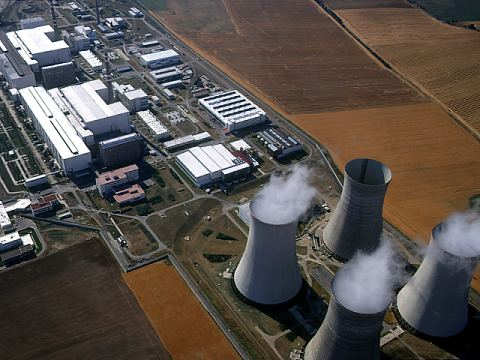
\includegraphics[width=0.37\linewidth]{edu02}};
         \node  [right=1.5cm of zona]   (kazeta)  {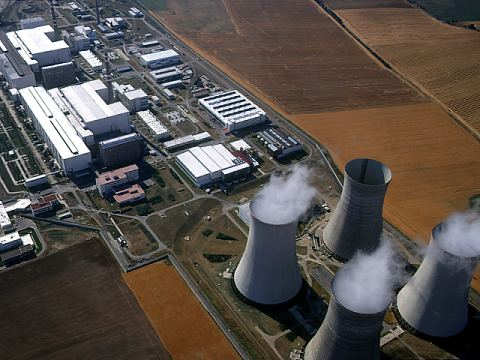
\includegraphics[width=0.37\linewidth]{edu02}};
         \draw
          let
            \p1 = (zona.south west),
            \p2 = (zona.south east)
          in
            node [below=.5cm of zona.south, text width={.9*(\x2-\x1)}, font=\footnotesize] (zonalbl) {Neutronový tok v $\frac16$ symetrie reaktoru};
            
        \draw
          let 
            \p1 = (kazeta.south),
            \p2 = (zonalbl)
          in
            (\x1,\y2) node [font=\footnotesize] (kazetalbl) {Neutronový tok ve vybrané kazetě};
      \end{tikzpicture}
    }
    \vspace{-0.25cm}
    \begin{center} Hermes \end{center}
  }
  
%%%%%%%%%%%%%%%%%%%%%%%%%%%%%%%%%%%%%%%%%%%%%%%%%%%%%%%%%%%%%%%%%%%%%%%%%%%%%%
%  \headerbox{Otevřené problémy}{name=problemy,column=1,below=vysledky,span=2}{
%%%%%%%%%%%%%%%%%%%%%%%%%%%%%%%%%%%%%%%%%%%%%%%%%%%%%%%%%%%%%%%%%%%%%%%%%%%%%%
%    \begin{itemize}
%      \item Problem 1
%      \item Problem 2
%      \item Problem 3
%    \end{itemize}    
%  }  
\end{poster}%
\end{document}
